\documentclass[]{article}

\usepackage[spanish]{babel}
\usepackage[table]{xcolor}
\usepackage{amsmath}
\usepackage{graphicx}
\usepackage{subcaption}
\usepackage{wrapfig}
\usepackage{lipsum}
\usepackage{amsmath}
\usepackage{amsfonts}
\usepackage{array}
\usepackage{multirow}
\usepackage{slashbox}
\usepackage{algpseudocode}
\usepackage{algorithm}
\usepackage{listings}

\renewcommand{\algorithmicrequire}{\textbf{Entrada: }}
\renewcommand{\algorithmicensure}{\textbf{Salida: }}

\renewcommand{\vector}[2]{\left( \begin{array}{c}
		#1 \\
		#2
	\end{array} \right)}

%\renewcommand{\ecuacioncuad}[3]{ #1 x^2 + #2 x + #3}

\newenvironment{ambiente}{\hrule \centering}{\hrule}


\newcounter{cteorema}
%\counterwithin{cteorema}{section}

\newenvironment{teorema}{ \refstepcounter{cteorema} \textbf{Teorema~\thecteorema .-}}{}

%\definecolor{name}{model}{color-spec}
\definecolor{codegreen}{rgb}{0,0.6,0}
\definecolor{codegray}{rgb}{0.5,0.5,0.5}
\definecolor{codepurple}{rgb}{0.58,0,0.82}
\definecolor{backcolour}{rgb}{0.95,0.95,0.92}


\lstdefinestyle{mystyle}{
	backgroundcolor=\color{backcolour},
	commentstyle=\color{codegreen},
	keywordstyle=\color{magenta},
	numberstyle=\tiny\color{codegray},
	stringstyle=\color{codepurple},
	basicstyle=\ttfamily\footnotesize,
	breakatwhitespace=false,         
	breaklines=true,                 
	captionpos=b,                    
	keepspaces=true,                 
	numbers=left,                    
	numbersep=5pt,                  
	showspaces=false,                
	showstringspaces=false,
	showtabs=false,                  
	tabsize=2
}

\lstset{style=mystyle}

%opening
\title{Borrador 1}
\author{Norberto}

\begin{document}

\maketitle

\begin{abstract}
Esto es un resumen.
\end{abstract}

\section{Sección 1}
\subsection{Subsección 1}

\section{Tamaños de letra}
Todos los comandos comienzan con $\backslash$.
tiny
scriptsize
footnotesize
small
normalsize
large
Large
LARGE
huge
Huge

\normalsize
Hola mundo
{\small Hola mundo 2}
Hola mundo 3

\section{Estilo de texto}
Itálicas
Negritas
Subrayado
%el siguiente texto está en itálicas (atajo ctrl + i)
\textit{Texto en itálicas.} 
\textit{Texto en itálicas 2}
%El siguiente texto está en negritas (atajo es ctrl+b)
\textbf{Texto en negritas.}
\textbf{Texto en negritas 2}

%El siguiente texto aparece subrayado.
\underline{Texto subrayado.}

%texto en itálicas, negritas y subrayado
\textit{\textbf{\underline{MEGA TEXTO}}}

\section{Color de texto.}
\textcolor{red}{Texto en color rojo.\\
	 Párrafo 2.}

\section{Alineación de texto}
% Texto centrado
\begin{center}
	Este texto aparecerá centrado.
\end{center}

\begin{flushright}
	Este texto aparecerá a la derecha.
\end{flushright}

\begin{flushleft}
	Este texto aparecerá a la izquierda.
\end{flushleft}

\section{Caracteres especiales}
El 35\% de los estudiantes reprobó \$ \\

$\backslash$ - sirve para la llamada de comandos
\$ - Sirve para generar modos matemáticos (escribir ecuaciones)
\# - Sirve para manejar argumentos dentro de macros y ambientes
\& - Sirve para tabular y realizar alineaciones. 

%para el manejo de símbolos de exclamación, interrogación y acentos
?` - signo de interrogación para abrir
!` - signo de exclamación para abrir
\'a - a acentuada
`entrecomillado simple'
``entrecomillado doble''

\section{Modos matemáticos.}
Modo matemático dentro de la línea donde se escribe $\alpha + \beta = 1$

Para poner la ecuación centrada. 
$$
	\alpha + \beta = 1
$$
\[
\alpha + \beta = 1
\]

\begin{equation*}
	\alpha + \beta = 1 \label{eq1}
\end{equation*}

La ecuación \ref{eq1} representa...

el límite:  $\lim_{x\rightarrow \infty}$ y $\displaystyle{\lim_{x\rightarrow \infty}}$
 
 \begin{align*}
 	x+y & = \alpha + \beta \\
 	& =\sqrt{x+y}
 \end{align*}

\[
\begin{array}{lcc}
	1 & 2 & 3 \\
	4 & 5 & 6 \\
	x^2 + y^2 &0 &0
\end{array}
\]

\[
A = \left(\begin{array}{lcc}
	1 & 2 & 3 \\
	4 & 5 & 6 \\
	x^2 + y^2 &0 &0
\end{array}\right)
\]

\[
	\begin{array}{rcl}
		x+y & = & 1\\
		2x +3y &=& 2\\
		\displaystyle{\sum_{i=1}^{n} x_{ij}} &=& 1 \hspace{3cm}   j\in J
	\end{array}
\]

Si queremos sólo un arreglo sin paréntesis:

\[
\begin{matrix}
	1 & 2 &3 \\
	4 & 5 & 6
\end{matrix}
\]
Si queremos paréntesis redondos (normales):

\[
\begin{pmatrix}
	1 & 2 &3 \\
	4 & 5 & 6
\end{pmatrix}
\]

Si queremos paréntesis corchetes:

\[
\begin{bmatrix}
	1 & 2 &3 \\
	4 & 5 & 6
\end{bmatrix}
\]

Si queremos paréntesis llaves:

\[
\begin{Bmatrix}
	1 & 2 &3 \\
	4 & 5 & 6
\end{Bmatrix}
\]

Si queremos paréntesis `valor absoluto':

\[
\begin{vmatrix}
	1 & 2 &3 \\
	4 & 5 & 6
\end{vmatrix}
\]

Si queremos paréntesis `normas':

\[
\begin{Vmatrix}
	1 & 2 &3 \\
	4 & 5 & 6
\end{Vmatrix}
\]

\section{Listas}

\begin{itemize}
	\item Primer elemento
	\item Segundo elemento
	\begin{itemize}
		\item Primer subelemento
		\item Segundo subelemento
	\end{itemize}
\end{itemize}

\begin{enumerate}
	\item Primer elemento $x+y$
	\item Segundo elemento
	\begin{enumerate}
		\item Primer subelemento
		\item Segundo subelemento
		\begin{itemize}
			\item 1
			\item 2
		\end{itemize}
	\end{enumerate}
\end{enumerate}

\section{Figuras}
Una de las instrucciones más importantes es el $\backslash$includegraphics que agrega gráficos existentes (en formato de imagen).

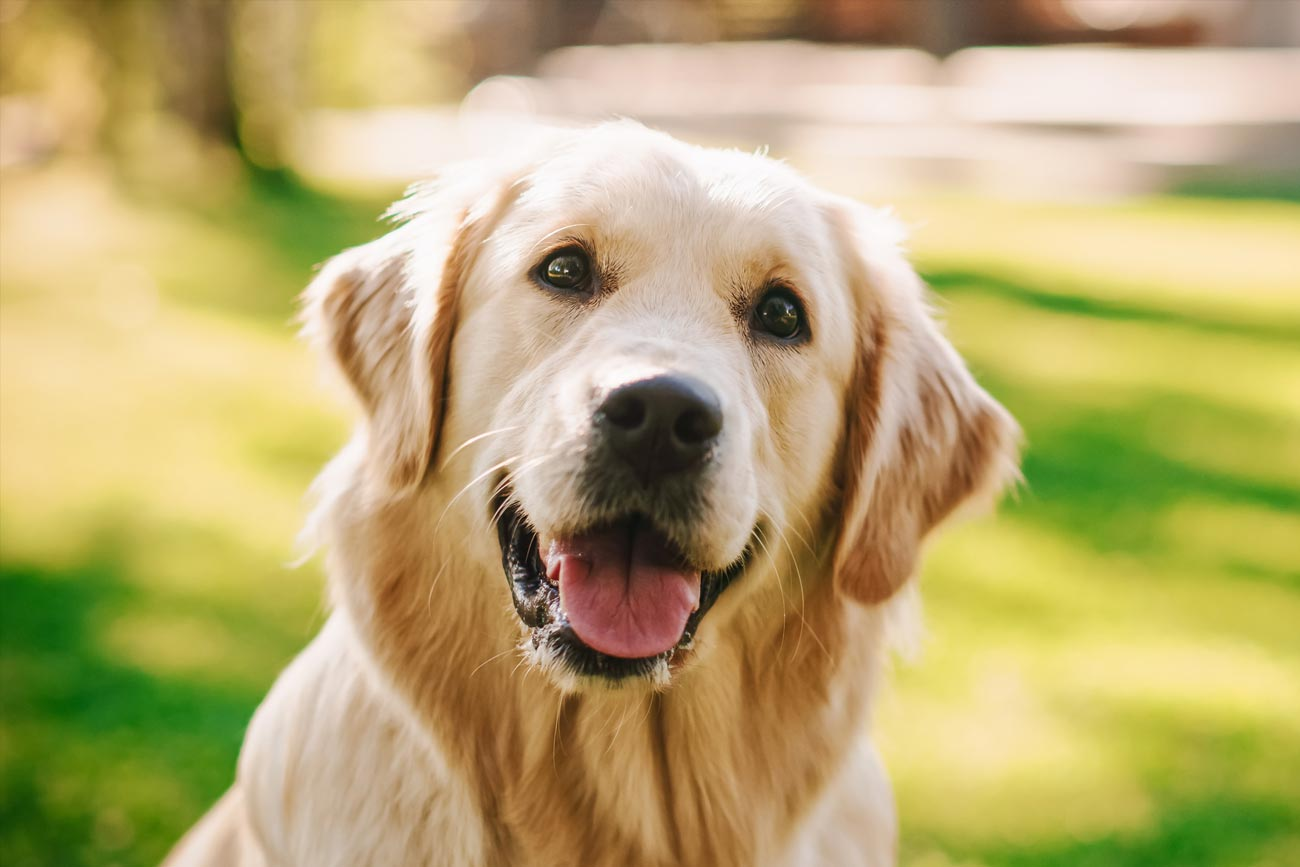
\includegraphics[width = 0.5\textwidth ]{perro1.jpg}

Para agregar pie a la imagen, sólo hay que agregar el gráfico a un entorno figure.

\begin{figure}
	\centering
	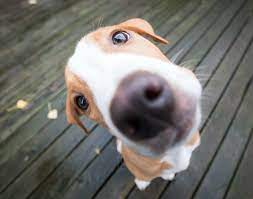
\includegraphics[width = 0.5\textwidth ]{perro2.jpg}
	\caption{Imagen del perro 2}
	\label{fig:perro2}
\end{figure}

El perro 2 se encuentra en la figura \ref{fig:perro2}.

\subsection{Posicionamiento de figuras}

\begin{itemize}
	\item h $\rightarrow$ intenta posicionar la imagen (tabla,...) en la misma posición en donde se encuentra el entorno figure.
	\item t $\rightarrow$ intenta posicionar la imagen en la parte superior de la página.
	\item b $\rightarrow$ intenta posicionar la imagen en la parte inferior de la página. 
	\item p $\rightarrow$ posiciona todas las imágenes en una página en específico. 
	\item ! $\rightarrow$ se utiliza en conjunto con cualquiera de los anteriores para forzar el posicionamiento.
	\item H $\rightarrow$ forza a posicionar el gráfico en la misma posición que el entorno figure y se encuentra en la librería float; es análogo a hacer h!.
\end{itemize}

\begin{figure}[h!]
	\centering
	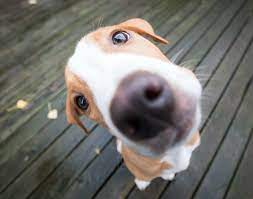
\includegraphics[width = 0.5\textwidth ]{perro2.jpg}
	\caption{Imagen del perro 2}
	\label{fig:perro2Pos}
\end{figure}

\begin{figure}
	\begin{subfigure}{0.5\textwidth}
		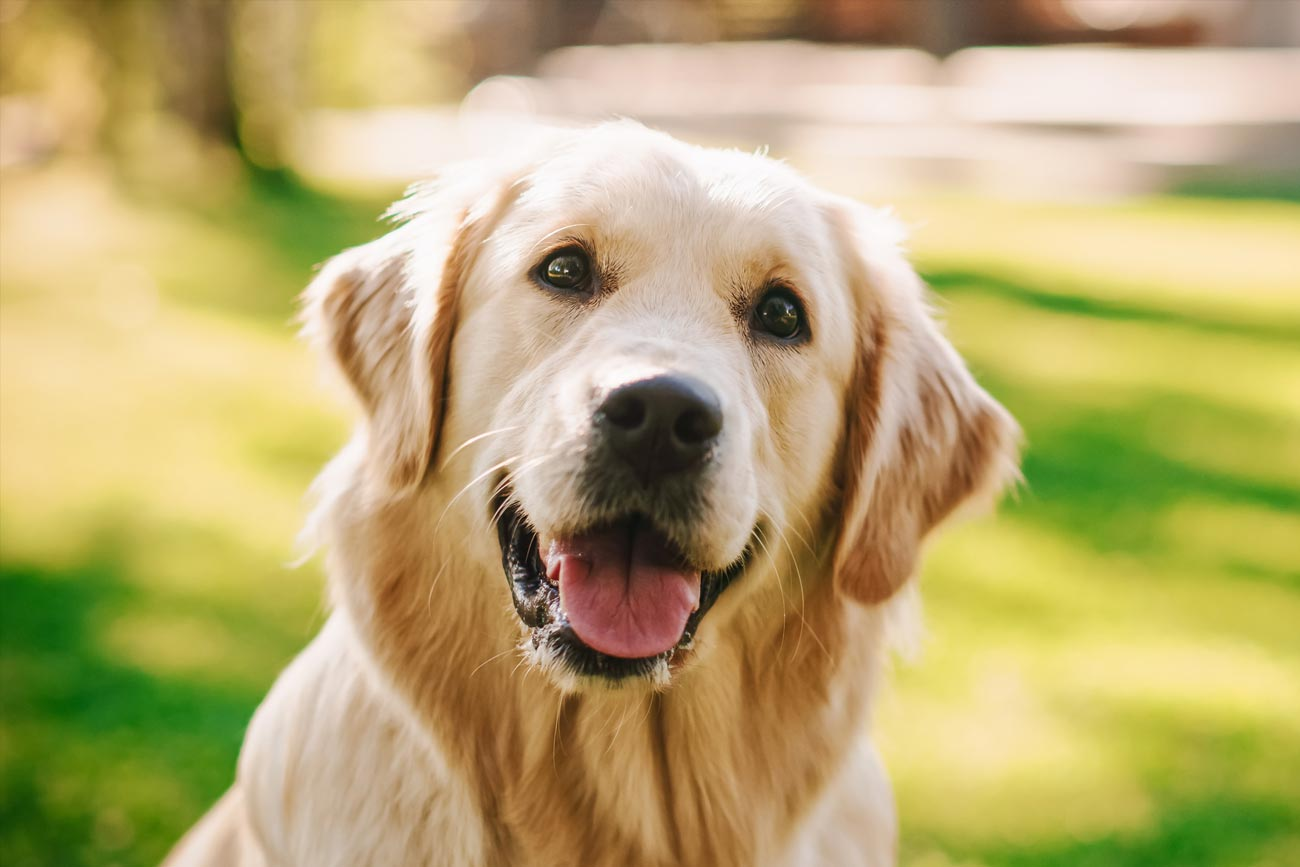
\includegraphics[width = \textwidth ]{perro1.jpg}
		\caption{perro 1}
	\end{subfigure}
	\begin{subfigure}{0.5\textwidth} 
		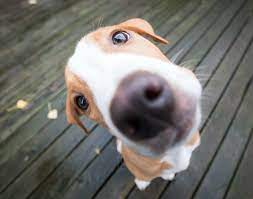
\includegraphics[width =\textwidth ]{perro2.jpg}
		\caption{perro2}
	\end{subfigure}
\caption{Imágenes de perros}
\end{figure}

\lipsum[1-5]

\begin{wrapfigure}{r}{0.5\textwidth}
	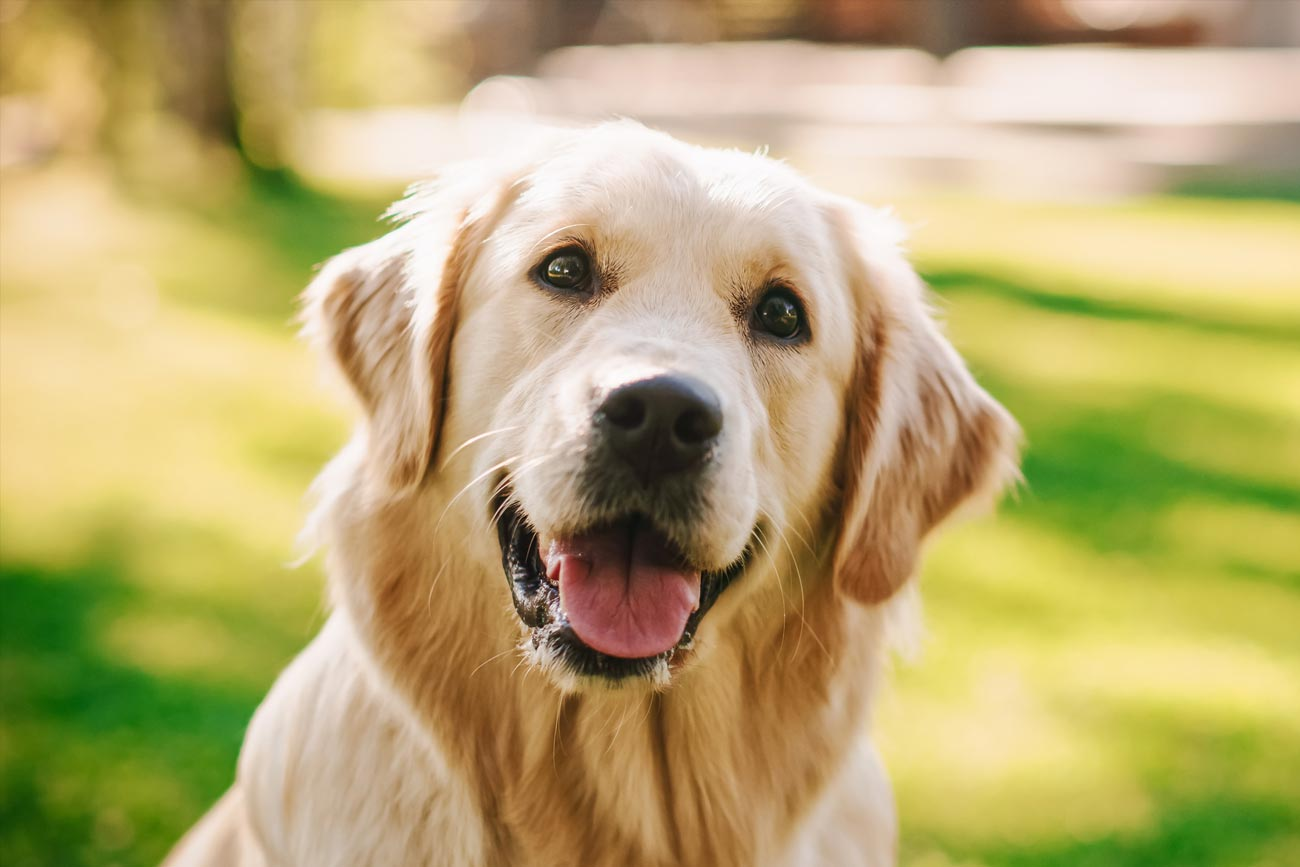
\includegraphics[width = 0.5\textwidth]{perro1.jpg}
\end{wrapfigure}

\lipsum[1-3]

\section{Tablas}

El entorno más importante para generar tablas en \LaTeX es `tabular'.

\begin{tabular}{cccc}%Cantidad de columnas y el posicionamiento del texto en columnas
	col1 & col2 & col3 & col4\\
	1	&	2	&	3	&	4\\
	5	&	6	&	7	&	8\\
\end{tabular}

Para agregar bordes verticales se utiliza $|$ al momento de definir las columnas y si se desea agregar bordes horizontales se usa $\backslash$hline.

\begin{tabular}{|cccc|}%Cantidad de columnas y el posicionamiento del texto en columnas
	\hline 
	col2 & col2 & col3 & col4\\
	\hline
	1	&	2	&	3	&	4\\
	5	&	6	&	7	&	8\\
	\hline
\end{tabular}

No sólo es posible definir el posicionamiento del texto en las columnas (horizontal), sino también dentro de las filas(vertical).

\begin{tabular}[c]{|cccc|}%Cantidad de columnas y el posicionamiento del texto en columnas
	\hline 
	col2 & col2 & col3 & col4\\ [1cm]
	\hline
	1	&	2	&	3	&	4\\
	5	&	6	&	7	&	8\\
	\hline
\end{tabular}

Para hacer celdas multilínea generar las columnas con posicionamientos m,p o b de la paquetería array.

\begin{tabular}{|b{1cm} ccc|}%Cantidad de columnas y el posicionamiento del texto en columnas
	\hline 
	hola cómo estás & col2 & col3 & col4\\ 
	\hline
	1	&	2	&	3	&	4\\
	5	&	6	&	7	&	8\\
	\hline
\end{tabular}

donde: 
\begin{itemize}
	\item m posiciona el texto en el centro de manera vertical.
	\item b posiciona el texto en la parte inferior de la celda.
	\item p posiciona el texto en la parte superior de la celda.
\end{itemize}

\subsection{Combinar celdas}

Para combinar celdas existen dos instrucciones  $\backslash$multicolumn y $\backslash$multirow. Particularmente, para la última instrucción es necesaria la paquetería multirow.

\begin{tabular}[c]{|c|c|c|c|}%Cantidad de columnas y el posicionamiento del texto en columnas
	\hline 
	\multicolumn{2}{|c|}{Col1 y col 2} &col3 &col4\\
	\hline
	col1 & col2 & col3 & col4\\
	\hline
	1	&	2	&	3	&	4\\
	\hline
	\multirow{2}{3cm}{ combinación de filas} &	6	&	7	&	8\\ \cline{2-4}
		&	6	&	7	&	8\\
	\hline
\end{tabular}

\subsection{Colorear tabla}

Para colorear tablas  \colorbox{red}{tenemos} las siguientes instrucciones:

\begin{itemize}
	\item $\backslash$rowcolors
	\item  $\backslash$rowcolor
	\item $\backslash$columncolor
	\item  $\backslash$cellcolor
\end{itemize}

{\rowcolors{2}{gray}{green}
\begin{tabular}[c]{|cccc|}%Cantidad de columnas y el posicionamiento del texto en columnas
	\hline 
	col2 & col2 & col3 & col4\\ [1cm]
	\hline
	1	&	2	&	3	&	4\\
	5	&	6	&	7	&	8\\
	1	&	2	&	3	&	4\\
	5	&	6	&	7	&	8\\
	1	&	2	&	3	&	4\\
	5	&	6	&	7	&	8\\
	\hline
\end{tabular}
}

\begin{tabular}[c]{|cccc|}%Cantidad de columnas y el posicionamiento del texto en columnas
	\hline 
	col2 & col2 & col3 & col4\\ [1cm]
	\hline
	\rowcolor{green}
	1	&	2	&	3	&	4\\
	5	&	6	&	7	&	8\\
	1	&	2	&	3	&	4\\
	5	&	6	&	7	&	8\\
	1	&	2	&	3	&	4\\
	5	&	6	&	7	&	8\\
	\hline
\end{tabular}

\begin{tabular}[c]{|c >{\columncolor{codegreen}}ccc|}%Cantidad de columnas y el posicionamiento del texto en columnas
	\hline 
	col2 & col2 & col3 & col4\\ [1cm]
	\hline
	1	&	2	&	3	&	4\\
	5	&	6	&	7	&	8\\
	1	&	2	&	3	&	\cellcolor{red!40}4\\
	5	&	6	&	7	&	8\\
	1	&	2	&	3	&	4\\
	5	&	6	&	7	&	8\\
	\hline
\end{tabular}

\subsection{Comando slash (celdas diagonales)}

\begin{tabular}[c]{|c >{\columncolor{codegreen}}ccc|}%Cantidad de columnas y el posicionamiento del texto en columnas
	\hline 
	\backslashbox{t1}{t2} & col2 & col3 & col4\\
	\hline
	1	&	2	&	3	&	4\\
	5	&	6	&	7	&	8\\
	1	&	2	&	3	&	\cellcolor{red!40}4\\
	5	&	6	&	7	&	8\\
	1	&	2	&	3	&	4\\
	5	&	6	&	7	&	8\\
	\hline
\end{tabular}

\subsection{Entorno table}

\begin{table}[!h]
	\centering
	\begin{tabular}{|c >{\columncolor{codegreen}}ccc|}%Cantidad de columnas y el posicionamiento del texto en columnas
		\hline 
		\backslashbox{t1}{t2} & col2 & col3 & col4\\
		\hline
		1	&	2	&	3	&	4\\
		5	&	6	&	7	&	8\\
		1	&	2	&	3	&	\cellcolor{red!40}4\\
		5	&	6	&	7	&	8\\
		1	&	2	&	3	&	4\\
		5	&	6	&	7	&	8\\
		\hline
	\end{tabular}
	\caption{Descripción de tabla}
	\label{tab:tabla1}
\end{table}

En la tabla \ref{tab:tabla1} se describe...

\section{Pseudocódigo}
Para escribir pseudocódigo se utilizará la paquetería algpseudocode. Entorno algorithm para agregar descripciones y etiquetas al algoritmo.

\begin{algorithm}[!h]
	\caption{Selection sort}
	\label{alg:SS}
	\begin{algorithmic}
		\Require $V$ vector de números enteros
		\Ensure $V$ ordenado descendente
		\State $V \leftarrow \mbox{\textbf{Crear\_vector}}(n)$ \Comment{$n$ es el tamaño del vector.}
		\For{$i = \overline{1:n}$}
		\State $(max, argmax) \leftarrow \max(V,i)$
		\State Intercambio$(V, i, argmax)$
		\EndFor \\
		\Return $V$
	\end{algorithmic}
\end{algorithm}

En el algoritmo \ref{alg:SS} la función \textbf{Crear\_vector} genera un vector aleatorio de números enteros.

\begin{algorithm}[!h]
	\caption{Selection sort}
	\label{alg:SS}
	\begin{algorithmic}
		\Require $V$ vector de números enteros
		\Ensure $V$ ordenado descendente
		\State $V \leftarrow \mbox{\textbf{Crear\_vector}}(n)$ \Comment{$n$ es el tamaño del vector.}
		\For{$i = \overline{1:n}$}
		\State $(max, argmax) \leftarrow \max(V,i)$
		\State Intercambio$(V, i, argmax)$
		\EndFor 
		\While{condition}
		\EndWhile
		\If{condition}
		\ElsIf{condition}
		\Else
		\EndIf \\
		\Return $V$
	\end{algorithmic}
\end{algorithm}

\section{Código}
Para agregar código al documento es necesario utilizar la paquetería linstings y el ambiente lstlisting.

\begin{lstlisting}[language= C++, caption=Hola mundo]
	#include <iostream>
	using namespace std;
	//Este codigo hace un hola mundo
	int main(){
		cout << "Hola mundo" << endl;
		return 0;	
	}
\end{lstlisting}


\begin{lstlisting}[language= Python, caption=Hola mundo]
	import pandas as pd
	print('hola mundo')
\end{lstlisting}


\section{Macros}

Generar comandos para objetos que no existen dentro de las paqueterías de latex y que van a ser utilizados constantemente dentro del documento.

Para generarlos se utiza el comando renewcommand{cmd}[args]{def}.

Un ejemplo de un vector en $\mathbb{R}^2$:

\[
	v = \vector{v_1}{v_2}
\]

otro ejemplo:

%\[
%	\ecuacioncuad{2}{3}{1}
%\]

\section{Ambientes propios}

Para generar los ambientes en latex se hace uso del comando neweviroment{nombre}[argumentos]{inicio} Contenido {final}


\begin{ambiente}
	hola mundo de latex
\end{ambiente}

\begin{teorema}
	hola
\end{teorema}

\begin{teorema}
	hola 2
\end{teorema}


\section{Gestión de bibliografía}
\begin{teorema}
	hola 3
\end{teorema}
\subsection{Manual}
%\cite{Ghosh-Dastidar2009} ...
%
%\begin{thebibliography}{}
%	\bibitem{Ghosh-Dastidar2009} Ghosh-Dastidar, S., Adeli, H. (2009). Spiking neural networks. International journal of neural systems, 19(04), 295-308.
%\end{thebibliography}

\subsection{Automática}
Utilizar Bibtex para agregar la bibliografía.

\cite{bishop1994neural}...

Estilos:
\begin{itemize}
	\item abbrv
	\item acm
	\item alpha
	\item apalike
	\item ieeetr
	\item plain
	\item siam
	\item unstr
\end{itemize}


\bibliographystyle{apalike}
\bibliography{refs}

\end{document}
